\section{Espais topològics 2AN i espais separables}

\begin{defi}
    Un espai topològic $X$ es diu que satisfà el segon axioma de numerabilitat (2AN) si té una base de cardinal numerable.
\end{defi}

\begin{example}
    Amb la topologia usual, $\real$ t\'e una base numerable: la fam\'ilia de tots els intervals oberts $(a, b)$ amb $a, b \in \q$. An\`alogament, també $\real^n$ té una base numerable:
    \[B=\left\{(a_1,b_1)\times\dots\times(a_n,b_n)\,|\,a_i, b_i\in \q, 1\leq i\leq n\right\}. \]
\end{example}

\begin{defi}
    Es diu que un conjunt $A$ és dens en $X$ si $\overline{A} = X$. Un espai s'anomena separable si té un subconjunt numerable dens.
\end{defi}

\begin{example}
    Tenim que $\overline{\q} = \real$. Com que $\q$ és numerable, $\real$ és separable. Més generalment, $\real^n$ és separable perquè admet $\q^n$ com a subconjunt dens.
\end{example}

\begin{prop}
    Un espai mètric $X$ és 2AN si i només si és separable.
\end{prop}
\begin{proof}
    Sigui $\B$ una base numerable de $X$. Per a cada $B \in \B$, prenem un punt $x_B \in B$ qualsevol. Llavors, com és fàcil de comprovar, el conjunt $\left\{x_B\right\}_{B \in \B}$ és dens.
    
    \quad
    
    Sigui $A$ un subconjunt numerable dens de l'espai. Llavors
    \[\B = \left\{B_{\sfrac{1}{n}} (a) \, | \, a\in A, \, n\in \n\right\}\]
    és una base numerable de l'espai. És numerable perquè és reunió numerable de conjunts numerables. A més, és una base ja que sigui $x$ un punt qualsevol i $U$ un entorn obert seu. Com que $x$ és interior a $U$, $\exists n>0$ tal que $B_{\sfrac{1}{2n}}(x)\cap A\subseteq U\cap A$. Provem que $x \in B_{\sfrac{1}{2n}}(a)\subseteq U$. Per la desigualtat triangular, sigui $y \in B_{\sfrac{1}{2n}}(a)$, es té
    \[d(x, y) \leq d(x, a) + d(a, y) < \frac{1}{2n} + \frac{1}{2n} = \frac{1}{n}\]
    i, per tant, $y\in B_{\sfrac{1}{n}}(x) \subseteq U$.
\end{proof}

\section{Topologia quocient}
\begin{obs}
    Siguin $X$ un conjunt i $\sim$ una relació d'equivalència, llavors $X/\sim$ \'es el conjunt de classes d'equivalència. Si $f\colon X\rightarrow Y$ exhaustiva, definim $x\sim x' \iff f(x) = f(x')$ i tenim que
    \begin{align*}
        \overline{f} \colon X/\sim &\rightarrow Y \\
        \left[ x \right] &\mapsto f(x)
    \end{align*}
    \'es bijectiva.
\end{obs}
\begin{defi}
    Sigui $X$ un espai topològic. Siguin $Y\in X$ i $\pi \colon X \rightarrow Y$ exhaustiva. Diem que $Y$ t\'e la topologia quocient per $\pi$ si els oberts de $Y$ són
    \[ \T_Y = \left\{ V\subseteq Y\,|\,\pi^{-1}(V) \in \T_X \right\}. \]
\end{defi}
\begin{prop}
    Propietats:
    \begin{enumerate}
        \item La topologia quocient de $Y$ per $\pi$ \'es la m\'es fina que fa $\pi$ contínua.
        \item Sigui $g\circ\pi \colon X \stackrel{\pi}{\rightarrow} Y \stackrel{g}{\rightarrow} Z$. $g$ \'es contínua $\iff g\circ\pi$ \'es contínua.
    \end{enumerate}
\end{prop}
\begin{proof}
    Vegem-ho.
    \begin{enumerate}
        \item Immediat per la definició de topologia quocient.
        \item La implicació cap a la dreta: $g \circ \pi$ \'es contínua perquè \'es composició de contínues.

            La implicació cap a l'esquerra: Sigui $W \subset Z$ obert, $g^{-1}(W) \subset Y$ \'es obert ja que
            \[\pi^{-1}\left( g^{-1}\left( W \right) \right) = \left( g\circ \pi \right)^{-1}\left( W \right) \implies \text{obert.}\]
    \end{enumerate}
\end{proof}
\begin{prop}[Tallar i enganxar]
    Siguin $f\colon X\rightarrow Y$ un homeomorfisme i $\sim_X$, $\sim_Y$ relacions d'equivalència a $X$ i a $Y$ tals que $x \sim_X x' \iff f\left( x \right) \sim_Y f\left( x' \right)$, llavors $f$ indueix un homeomorfisme $\overline{f} \colon X/\sim \rightarrow Y/\sim$.
\end{prop}
\begin{proof}
    Com que $x\sim x' \implies f\left( x \right) \sim f\left( x' \right)$, $f$ indueix una aplicació $\overline{f}\colon X/\sim \rightarrow Y/\sim$ que fa commutatiu el diagrama
        \[
            \begin{tikzcd}
                X\ar{r}{f}\ar{d}[swap]{p} & Y\ar{d}[swap]{q}\\[2ex]
                X/\sim \ar{r}{\overline{f}} & Y/\sim
            \end{tikzcd}
        \]
        Com que $q\circ f$ \'es contínua, per la propietat universal de la topologia quocient de $X/\sim$, $\overline{f}$ \'es contínua. Si $f$ \'es bijectiva, com que $x\sim x' \iff f\left( x \right) \sim f\left( x' \right)$, $\overline{f}$ \'es bijectiva. Apliquem el mateix raonament a $f^{-1}$ per deduir que $\overline{f}^{-1}$ \'es contínua.
\end{proof}
\begin{example}
    \begin{enumerate}
        \item[] 
        \item
            \[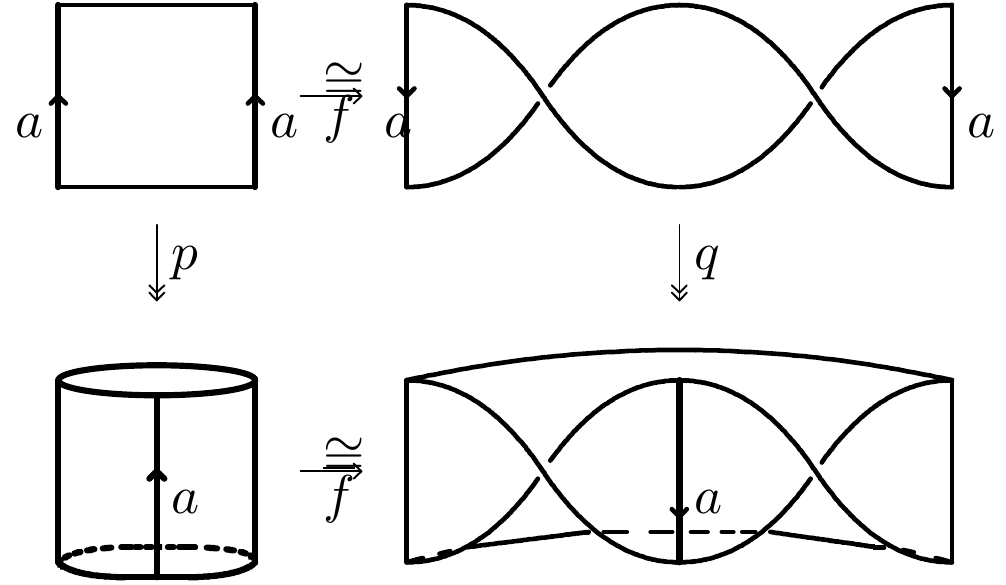
\includegraphics[scale=0.2]{figs_resum/cilindre.png}\]
        \item $\mathbb{D} = \left\{ \left( x, y \right) \,|\, x^2 + y^2 \leq 1 \right\}$
            \begin{multicols}{2}
                \[
                    \begin{tikzcd}
                        \mathbb{D}\ar{dr}\ar{d} & \\[2ex]
                        \mathbb{D}/\sim \ar{r}{\cong} & \mathbb{S}^2
                    \end{tikzcd}
                \]
                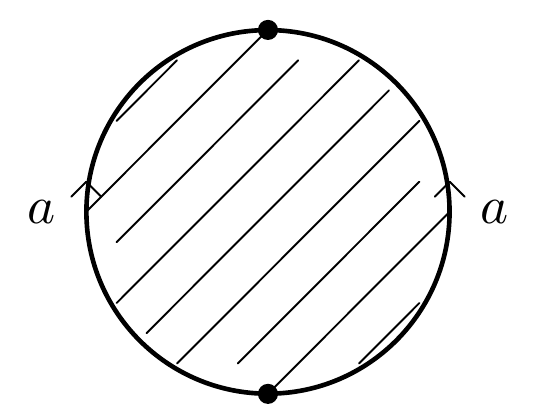
\includegraphics[scale=0.15]{figs_resum/esfera.png}
            \end{multicols}
        \item Altres: banda de Möbius, pla projectiu, ampolla de Klein, tor...
    \end{enumerate}
\end{example}

\section{Espai compacte i compacitat del producte}

\begin{defi}
    Un espai topològic $X$ és compacte si per tot recobriment obert $\mathscr{U}$ existeix un subrecobriment $\mathscr{V}\subset\mathscr{U}$ finit.
\end{defi}

\begin{lema}[Lema del tub]
    Siguin $X$ i $Y$ espais topològics, $Y$ compacte. Sigui $x\in X$ i $N$ obert de $X \times Y$ tal que $x\times Y \subset N$.
    Aleshores existeix $W \subset X$ obert tal que $x\times Y \subset W \times Y \subset N$.
\end{lema}
\begin{proof}
    Per cada punt $(x,y) \in x\times Y$ prenem un obert $U_y\times V_y$ de la base de $X\times Y$ que el contingui, de manera que $(U_y\times V_y) \subset N$. El conjunt de tots els $U_y\times V_y$ és un recobriment obert de $x_0\times Y$.
    
    $x \times Y \cong Y$ és compacte, del recobriment anterior se'n pot extraure un de finit $(U_1 \times V_1) \cup\dots\cup (U_n \times V_n)$.
    
    El conjunt $W = U_1 \cap\dots\cap U_n$ és obert de $X$ perquè és intersecció finita d'oberts, i $x \times Y \subset W\times Y \subset (U_1 \times V_1 \cup\dots\cup U_n \times V_n) \subset N$.
\end{proof}

\begin{prop}
    $X$, $Y$ espais topològics i $X \times Y$ la topologia producte. Aleshores
    \[X \times Y \text{ compacte } \Longleftrightarrow X,Y \text{ compactes}\]
\end{prop}
\begin{proof}
    Si $X \times Y$ és compacte i la projecció $\pi_X\!: X \times Y \rightarrow X$ és contínua, $\pi_X(X\times Y)=X$ és compacte. Anàlogament per $Y$.
    
    \quad
    
    Suposem que $X$ i $Y$ són compactes. Sigui $\mathscr{U}$ un recobriment obert de $X \times Y$. $x \times Y$ és compacte, per tant hi ha un recobriment finit $x \times Y \subset V_1 \cup\dots\cup V_n$ amb elements de $\mathscr{U}$.
    
    Considerem $N = V_1 \cup\dots\cup V_n$, pel lema del tub existeix un $x \in W \subset X$ tal que $x\times Y \subset W \times Y \subset N$. Per tant $(W \times V_1) \cup\dots\cup (W \times V_n)$ és un recobriment obert finit de $W \times Y$ amb elements de $\mathscr{U}$.
    
    Ara, per cada $x\in X$ apliquem el lema del tub i obtenim un $x \in W_x$ tal que $W_x \times Y$ té un recobriment finit amb elements de $\mathscr{U}$. Els $W_x$ formen un recobriment de $X$, i $X$ és compacte, tenim un recobriment finit $X = W_1 \cup\dots\cup W_n$. Per cada $W_i$ prenem els $V$ corresponents i obtenim un subrecobriment de $\mathscr{U}$ finit, per tant $X\times Y$ és compacte.
    
\end{proof}


\section{Tancats, Hausdorff i compacitat}

\begin{defi}
    Un espai topològic $X$ \'es Hausdorff si $\forall \: x, y \in X, \, \exists \: U,\, V$
    oberts tals que $U \cap V = \varnothing$ i $x \in U,\, y \in V$.
\end{defi}
\begin{prop}
   Tot supespai tancat d'un espai compacte \'es un espai compacte. 
\end{prop}
\begin{proof}
    Siguin $X$ un espai compacte, $Y \subseteq X$ un tancat i $\mathcal{U}$ un recobriment
    de $Y$ per oberts de $X$. Afegint l'obert $X \setminus Y$ obtenim un 
    recobriment obert de $X$ que, per ser $X$ compacte, cont\'e un 
    subrecobriment finit. Els oberts d'aquest subrecobriment diferents 
    de $X \setminus Y$  han de cobrir $Y$, i per tant formen un subrecobriment finit de 
    $\mathcal{U}$.
\end{proof}
\begin{example}
    La recta real amb la topologia de complements finits \'es un espai compacte i tamb\'e ho
    \'es qualsevol subespai d'aquesta, però nom\'es són tancats els conjunts finits de punts,
    d'on un subespai compacte pot no ser tancat.
\end{example}
\begin{prop}
    Tot subespai compacte d'un espai de Hausdorff \'es tancat.
\end{prop}
\begin{proof}
    Siguin $X$ un espai de Hausdorff i $Y \subseteq X$ un subconjunt compacte. Vegem que
    $X \setminus Y$ \'es obert comprovant que tot punt $x_0 \in X \setminus Y$ \'es interior. Com $X$
    \'es de Hausdorff, per a cada $y \in Y$ existeixen oberts disjunts $U_y, V_y$ tals
    que $x_0 \in U_y, y \in V_y$.

    La família $\{V_y\}_{y \in Y}$ forma un recobriment obert de $Y$. Per ser $Y$ compacte,
    cont\'e un subrecobriment finit $Y \subseteq V_{y_1} \cup \dots \cup V_{y_n}$.
    Considerem els oberts
    \[ 
        V = V_{y_1} \cup \dots \cup V_{y_n}, \,
        U = U_{y_1} \cap \dots \cap U_{y_n},
    \]
    que són disjunts ja que si $z \in V$, aleshores 
    existeix $y_i$ tal que $z \not\in U_{y_i}$,
    d'on $z \not\in U$. Per tant, $U \subseteq X \setminus Y$.
\end{proof}
\begin{prop}
   Sigui $f : X \longrightarrow Y$ una aplicació contínua i bijectiva. Si $X$ \'es compacte
   i $Y$ \'es de Hausodrff, aleshores $f$ \'es un homeomorfisme.
\end{prop}
\begin{proof}
    Hem de provar $f^{-1}$ \'es contínua, però això \'es equivalent a que $f$ sigui tancada. 
    Sigui $C$ un tancat de $X$. Com $X$ \'es compacte, $C$ tamb\'e ho \'es. Per ser imatge
    d'un compacte per una aplicació contínua, $f(C)$ \'es compacte i per la
    proposició anterior, com $Y$ \'es de Hausdorff, tamb\'e \'es tancat.
\end{proof}


\section{Índexos}


\section{Superfícies}

\begin{def}[Varietat]
    Sigui $M$ un espai topològic. Direm que $M$ és una varietat de dimensió $n$ si:
    \begin{enumerate}[i)]
	\item $M$ es Haussdorff
	\item $M$ es $2AN$
	\item $\forall x \in M$, $\exists U \ni x$ obert i un homeomorfisme
	    $\phi \colon U \to \real^n$ ($M$ localment homeomorf a $\real^n$)
    \end{enumerate}
\end{def}

\begin{example}
    \begin{enumerate}
	\item $n = 1$, son corbes, per example $\real$ o $\mathbb{S}$. Mes en general:
	    \begin{itemize}
		\item No s'admenten autointerseccions
		\item No podem afegir límits (extrems) a les corbes.
	    \end{itemize}
	\item $n = 2$ , son superfícies.
	    % TODO poner pantallaso rico papi
	\item Que $M$ hagi de ser Haussdorff i $2AN$ és per evitar patologies (como el punts
	    dobles) y a més, ens permet triangular
	\item superfícies poligonals: $\mathbb{T}$, $\mathbb{K}$ (són ompactes i convexes)
	\item superfícies estàndar: superfícies poligonals corresponents a les paraules.
    \end{enumerate}
\end{example}

\begin{teo*}[C]
    Tota superfícies $S$ compacta i connexa és homeomorfa a una única superfície estàndar.
    \begin{itemize}
	\item $A_0 \colon aa^{-1} (g = 0) \rightarrow A_0 \cong \mathbb{S}^2$
	\item $A_g \colon a_1b_1a^{-1}_1 b^{-1}_1 \cdots a_gb_ga^{-1}_gb^{-1}_g (g \geq 1)
	    \rightarrow A_g \cong g \mathbb{T}$ ($g$-tors)
	\item $B_g \colon a_1a_1 \cdots a_ga_g (g \geq 1) \rightarrow B_g \cong g \mathbb{P}^2$
	    ($g$-plans projectius)
	\item
    \end{itemize}
    ($g$ és el gènere de la superfície)
\end{teo*}

\begin{def}[Orientabilitat]
    $S$ és no orientable si conté una cinta de Möbius. $S$ és orientable en cas contrari.
\end{def}

\begin{example}
    \begin{enumerate}
	\item $g \Po^2$, $g \geq 1$ NO és orientable.
	\item $g \mathbb{T}^2$, $g \geq 0$ sí que és orientable. ($g = 0$, $A_0 \leadsto \mathbb{S}^2$)
	\item $S \cong S^\prime \implies $ tenen la matteixa orientabilitat. De fet, dues superfícies
	    són homeomorfes si tenen el mateix gènere i la mateixa orientabilitat.
    \end{enumerate}
\end{example}

\begin{def}[Característia d'Euler]
    Sigui $(S, T)$ superfície triangulada, definim la caacterística d'Euler de $T$ per
    \[
        \psi (S, T) = v - a + c
    \]
    Donde $v$ són els vèrtex, $a$ les arestes i $c$ les cares.
\end{def}

\begin{teo*}
    $\psi(S)$ és independent de la tringulació.
\end{teo*}

\begin{example}
    \begin{enumerate}
	\item $\psi$
    \end{enumerate}<++>
\end{example}<++>
